\documentclass[
	fontsize=10pt, % Base font size
	twoside=false, % Use different layouts for even and odd pages (in particular, if twoside=true, the margin column will be always on the outside)
	open=any, % If twoside=true, uncomment this to force new chapters to start on any page, not only on right (odd) pages
	%chapterprefix=true, % Uncomment to use the word "Chapter" before chapter numbers everywhere they appear
	%chapterentrydots=true, % Uncomment to output dots from the chapter name to the page number in the table of contents
	numbers=noenddot, % Comment to output dots after chapter numbers; the most common values for this option are: enddot, noenddot and auto (see the KOMAScript documentation for an in-depth explanation)
	%draft=true, % If uncommented, rulers will be added in the header and footer
	%overfullrule=true, % If uncommented, overly long lines will be marked by a black box; useful for correcting spacing problems
]{kaobook}

% Set the language
\usepackage[english]{babel} % Load characters and hyphenation
\usepackage[english=american]{csquotes} % English quotes

\usepackage{lipsum}
\usepackage{tikz}
\usepackage{circuitikz}
\usepackage{tikz-timing}
\usepackage{nicefrac}
\usepackage{subcaption}
\usepackage{pgfplots}
\usepackage{listings}
\usepackage{fontawesome5}

%%% All colors used

\definecolor{gr10}{HTML}{e6e6e6}
\definecolor{gr20}{HTML}{cccccc}
\definecolor{gr30}{HTML}{b3b3b3}
\definecolor{gr40}{HTML}{999999}
\definecolor{gr50}{HTML}{808080}
\definecolor{gr60}{HTML}{666666}
\definecolor{gr70}{HTML}{4d4d4d}
\definecolor{gr80}{HTML}{333333}
\definecolor{gr90}{HTML}{191919}

%%% Sans serif font
\renewcommand{\familydefault}{\sfdefault}

%%% Setup for flowcharts

\usetikzlibrary{shapes.geometric, arrows, fit}
\tikzstyle{startstop} = [rectangle, rounded corners, minimum width=3cm, minimum height=1cm,text centered, draw=black, fill=gr40]
\tikzstyle{process} = [rectangle, minimum width=3cm, minimum height=1cm, text centered, draw=black, fill=gr20]
\tikzstyle{command} = [rectangle, minimum width=3cm, minimum height=1cm, text centered, draw=black, fill=gr10]
\tikzstyle{decision} = [diamond, minimum width=3cm, minimum height=1cm, aspect=1.5, text centered, draw=black, fill=gr30]
\tikzstyle{arrow} = [thick,->,>=stealth]

%%% For material score
\newcommand{\outerradius}{1cm}
\newcommand{\innerradius}{.75cm}
\newcommand{\barlength}{2cm}
\newcommand{\barheight}{1.5mm}
\newcommand{\barypos}[1]{- \outerradius + #1 * \outerradius / 2 - \outerradius / 4 - \barheight / 2}

\newcommand{\materialscore}[6]{
\begin{tikzpicture}

    \fill[gr20] (0,0) circle (\outerradius);
    \fill[gr50] (0,0) -- (0, \outerradius)
      arc (90:90-36*#2:\outerradius) -- (0,0);
    \fill[white] (0,0) circle (\innerradius);

     \node[gr70] at (\outerradius + 5mm, \barypos{4} + \barheight / 2) {\faIcon{magnet}};
     \fill[gr20] (\outerradius + 9mm, \barypos{4}) rectangle ++(\barlength, \barheight);
     \fill[gr50] (\outerradius + 9mm, \barypos{4}) rectangle ++(\barlength * 0.1 * #3, \barheight);

    \node[gr70] at (\outerradius + 5mm, \barypos{3} + \barheight / 2) {\faIcon{fire}};
    \fill[gr20] (\outerradius + 9mm, \barypos{3}) rectangle ++(\barlength, \barheight);
    \fill[gr50] (\outerradius + 9mm, \barypos{3}) rectangle ++(\barlength * 0.1 * #4, \barheight);

    \node[gr70] at (\outerradius + 5mm, \barypos{2} + \barheight / 2) {\faIcon{euro-sign}};
    \fill[gr20] (\outerradius + 9mm, \barypos{2}) rectangle ++(\barlength, \barheight);
    \fill[gr50] (\outerradius + 9mm, \barypos{2}) rectangle ++(\barlength * 0.1 * #5, \barheight);

    \node[gr70] at (\outerradius + 5mm, \barypos{1} + \barheight / 2) {\faIcon{eye}};
    \fill[gr20] (\outerradius + 9mm, \barypos{1}) rectangle ++(\barlength, \barheight);
    \fill[gr50] (\outerradius + 9mm, \barypos{1}) rectangle ++(\barlength * 0.1 * #6, \barheight);

    \foreach \l in {1,...,4}{
      \foreach \p in {1,...,9}{
        \draw[gr20, ultra thick] (\outerradius + 9mm + \barlength / 10 * \p, \barypos{\l}) -- ++(0, \barheight);
      }
    }

    \foreach \a in {0,36,72,...,360}{
      \draw[gr20, ultra thick] (\a+18:\innerradius) -- (\a+18:\outerradius);
    }

    \node at (\outerradius / 2 + \barlength / 2, \outerradius * 1.25){\large{\textbf{#1}}};
\end{tikzpicture}}

\usepackage{array} % for custom conditions environment

\newenvironment{conditions}
  {\par\vspace{\abovedisplayskip}\noindent\begin{tabular}{>{$}l<{$} @{${}={}$} l}}
  {\end{tabular}\par\vspace{\belowdisplayskip}}

% Load packages for testing
%\usepackage{blindtext}
%\usepackage{showframe} % Uncomment to show boxes around the text area, margin, header and footer
%\usepackage{showlabels} % Uncomment to output the content of \label commands to the document where they are used

% Load the bibliography package
\usepackage{styles/kaobiblio}
\addbibresource{main.bib} % Bibliography file

% Load mathematical packages for theorems and related environments. NOTE: choose only one between 'mdftheorems' and 'plaintheorems'.
\usepackage{styles/mdftheorems}
%\usepackage{styles/plaintheorems}

\graphicspath{{examples/documentation/images/}{images/}} % Paths in which to look for images

\makeindex[columns=3, title=Alphabetical Index, intoc] % Make LaTeX produce the files required to compile the index

\makeglossaries % Make LaTeX produce the files required to compile the glossary

\makenomenclature % Make LaTeX produce the files required to compile the nomenclature

% Reset sidenote counter at chapters
%\counterwithin*{sidenote}{chapter}

%----------------------------------------------------------------------------------------

\begin{document}

%----------------------------------------------------------------------------------------
%	BOOK INFORMATION
%----------------------------------------------------------------------------------------

%\titlehead{The \texttt{kaobook} class}
\subject{Diploma Thesis}

\title{Class-E Tesla Coil}
%\subtitle{Customise this page according to your needs}

\author{Marcher Simon\\Peyer Kassandra\\Felix Hamrle}

\date{\today}

%----------------------------------------------------------------------------------------

\frontmatter % Denotes the start of the pre-document content, uses roman numerals


%----------------------------------------------------------------------------------------
%	OUTPUT TITLE PAGE AND PREVIOUS
%----------------------------------------------------------------------------------------

% Note that \maketitle outputs the pages before here

% If twoside=false, \uppertitleback and \lowertitleback are not printed
% To overcome this issue, we set twoside=semi just before printing the title pages, and set it back to false just after the title pages
\KOMAoptions{twoside=semi}
\maketitle
\KOMAoptions{twoside=false}

%----------------------------------------------------------------------------------------
%	AFFIDAVIT
%----------------------------------------------------------------------------------------

\chapter*{Affidavit}
\addcontentsline{toc}{chapter}{Affidavit}

I declare in lieu of an oath that I have written the present thesis independently
and without outside help other than the stated sources, and that I have made the
passages taken from these sources recognisable as such.


%----------------------------------------------------------------------------------------
%	TABLE OF CONTENTS & LIST OF FIGURES/TABLES
%----------------------------------------------------------------------------------------

\begingroup % Local scope for the following commands

% Define the style for the TOC, LOF, and LOT
%\setstretch{1} % Uncomment to modify line spacing in the ToC
%\hypersetup{linkcolor=blue} % Uncomment to set the colour of links in the ToC
\setlength{\textheight}{23cm} % Manually adjust the height of the ToC pages

% Turn on compatibility mode for the etoc package
\etocstandarddisplaystyle % "toc display" as if etoc was not loaded
\etocstandardlines % toc lines as if etoc was not loaded

\tableofcontents % Output the table of contents

\listoffigures % Output the list of figures

% Comment both of the following lines to have the LOF and the LOT on different pages
\let\cleardoublepage\bigskip
\let\clearpage\bigskip

\listoftables % Output the list of tables

\endgroup

%----------------------------------------------------------------------------------------
%	MAIN BODY
%----------------------------------------------------------------------------------------

\mainmatter % Denotes the start of the main document content, resets page numbering and uses arabic numbers
\setchapterstyle{kao} % Choose the default chapter heading style

\pagelayout{wide} % No margins
\addpart{The Tesla Coil}
\pagelayout{margin} % Restore margins
\setchapterstyle{kao}
\setchapterpreamble[u]{\margintoc}

\chapter{Theory of Operation} % How it should work in theory
\labch{tc-theory-of-operation}

The tesla coil was invented by Nikola Tesla in 1891. His vision was to use this technology to wirelessly transmit power to people all over the world. While his plans didn't meet the expectations by far, he still opened up a whole new field of physics, which today helps power the modern world.

Tesla coils come in a huge variety of sizes, power and modes of operation. From simple spark gap tesla coils, which consist of only a few passive components, to solid state tesla coils, whose only limitations are one's technical skills, every single one amazes anew by combining the world of High Voltage and High Frequency.

In order to understand the class E topology which this thesis is about, we have to understand the basics first. 

\section{The Tesla Resonator}

A tesla resonator, also called tesla coil, is a resonant transformer consisting of two loosely coupled air-cored windings: the primary and secondary coil. The primary coil, hooked up to the driver circuit on one side and grounded on the other, is usually made out of every few turns of thick wire. It is placed around the bottom of the secondary coil, either shaped like an flat spiral, a concentric cylinder, or at any angle in between. The secondary coil on the other hand has a lot more turns and is a lot higher.

\begin{marginfigure}[*-5]
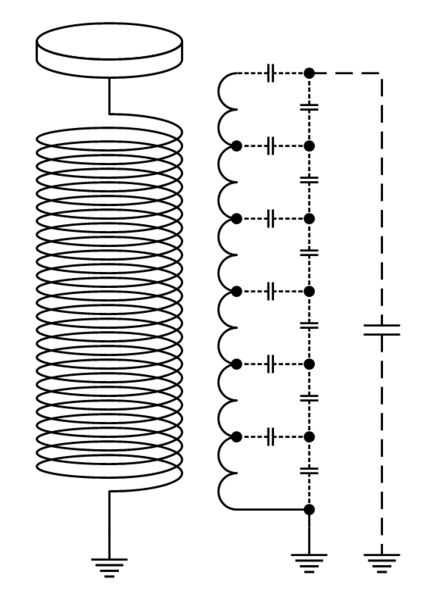
\includegraphics[width=\textwidth]{simon/resources/teslaCoilStrayCapacitance.png}
\caption{Stray capacitances of the secondary coil}
\labfig{teslaCoilStrayCapacintance}
\end{marginfigure}

As every real component, a coil has parasitic effects. The one relevant to a tesla coil's operation is the parasitic capacitance. A capacitance is just two different isolated voltage potentials, which is exactly, what we have along every single winding of a coil. This makes clear that every coil is actually an LC oscillator. The lower the inductance and capacitance of the coil, the higher the resonant frequency. This means that in order to lower the frequency to the desired one, many tesla coils have a top load, which, amongst others, acts like as an additional capacity towards ground.

If a high voltage, whose frequency is the resonant frequency of the secondary, is now applied to the primary coil, the LC circuit in the secondary coil starts oscillating and a very high voltage builds up gradually. Depending on the size and power of the tesla coil, this voltage can range from a few thousand to a few million volts. Once the voltage is high enough to ionise the air around the top\sidenote{This usually happens at a designated spark point}, it quickly discharges and the cycle starts over again.

\section{Exciting The Resonator}

There are various circuits which can be used for the excitation of the coil. Depending on the desired spark length, size\sidenote{The size of the secondary coil mostly determines its resonant frequency}, sensitivity to external effects, noise level and efficiency, different tesla coil drivers can be used. While Tesla's coils all used a spark gap topology, today we are able to use solid state devices to control the coil instead.

\subsection{The Spark Gap Tesla Coil}

\begin{marginfigure}
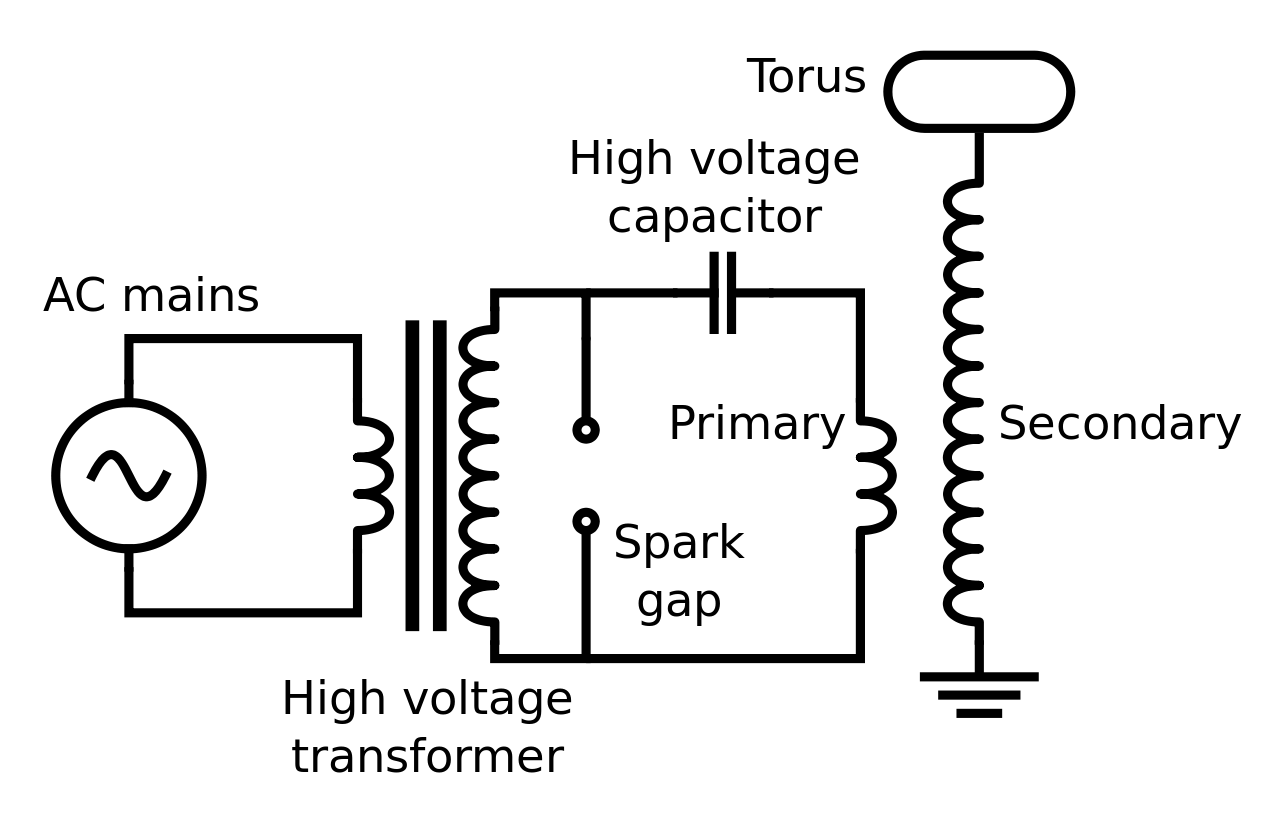
\includegraphics[width=\textwidth]{simon/resources/sparkGapTeslaCoil.png}
\caption{A simple spark gap tesla coil}
\labfig{sparkGapTeslaCoil}
\end{marginfigure}

The simplest and oldest of all drivers is the spark gap driver. In the first stage, the 230V mains voltage is transformed to a few kilovolts. Neon sign or microwave transformers are popular choices for this task. The capacitor gets charged up until the voltage is high enough to break through the spark gap. The spark gap then has a very low resistance and allows the current to oscillate between the capacitor and the primary coil. This oscillation frequency is usually in the order of ten to hundred kilohertz and is the same frequency as the resonant frequency of the secondary coil. In every cycle, a little energy is transferred to the secondary via the magnetic coupling of the coils. When the voltage in the secondary gets too high, a breakout occurs. This can happen one or more times within a period of the AC mains voltage. Once all the energy in the primary circuit has been transferred to the secondary or dissipated as heat, the spark gap \enquote{quenches} allowing the capacitor to charge up again.

Today, spark gap tesla coils are mostly only used for educational purposes anymore. Due to their many \textbf{disadvantages} they are avoided when power efficiency and noise level play a role. The disadvantages most worth mentioning include:

\begin{itemize}
\item A spark gap dissipates a lot of power, part of it as heat and part of it in creating a ozone, which also poses a health hazard, when operated in closed rooms.
\item The rapid igniting and quenching of the spark gap creates a lot of noise.
\item The whole operation cycle only depends on passive component values, which makes it very hard to control the power output and other characteristics.
\end{itemize}

\subsection{Solid State Tesla Coils}

Aside from vacuum tube tesla coils, which have existed before, semiconductor technology\sidenote{Unlike relays or hard disk drives, their semiconductor counterparts have no moving components. Hence the name \enquote{solid state}.} opened up a whole new world of possibilities for tesla coils. It was now possible to build up sophisticated amplifier circuits to excite the primary coil. Some of them still rely on resonant circuits, others use feedback loops to self-excite the primary coil, and again others use \glspl{ic} to control the driver.

The most common solid state topologies include:
\begin{itemize}
\item Slayer exciter
\item Half-bridge / full-bridge (single or dual resonant)
\item Class E
\end{itemize}

\subsubsection{Slayer Exciter Circuit}

The slayer exciter topology is the most common under hobbyist coilers\sidenote{This is how people building tesla coils often call themselves}, because it's by far the simplest one, only consisting of very few components. At it's hard sits the Transistor T controlling the current through the primary coil L1. When first powering on the circuit, current flows through R into the base of T, allowing current to flow through L1, creating a magnetic field.\sidenote{Since the magnetic field flows through both coils in the same direction, the winding direction of the secondary has to be reversed so that the output voltage won't be reversed.} The rapid change in the field induces a high voltage in the secondary coil L2. The parasitic capacitance C of L2 however only lets the voltage across it rise slowly, therefore pushing the potential of the bottom of the lower end of L2 to a negative voltage. As soon as the voltage falls below -0.7V, the diode D starts conducting and limits the negative voltage while providing current to charge up C\sidenote{The diode could be left out, since the base emitter junction also acts as diode, but in the most cases this damages the transistor}. Additionally, since the base emitter voltage is now negative, T stops conducting. This causes the magnetic field to start collapsing, causing the potential at the base to slowly rise, until T starts conducting again. The circuit is now in it's initial state, except that C is now charged to a high voltage and the process starts over again.

Since the timing of the circuit only depends on the values of L1, L2, and C, the circuit tunes itself, which makes it very stable to operate. But because of its simplicity it comes with a few disadvantages. Firstly, when T is conducting, it basically shorts L1, which leads to a high current and therefore power dissipated in T. This power can be reduced by choosing R to be rather high. This reduces the base current and therefore also the collector current. While this helps reducing the power dissipation it also reduces the output power of the coil. With a bit of extra complexity this circuit can however be made more efficient.

\begin{figure}[h!]
\centering
\begin{circuitikz}[european, american inductors]
  \draw (2,4) to[short, *-] (0,4) to[battery, l=V] (0,0) node[ground]{};
  \draw (2,4) to[R, l=R] (2,1) to[D-, l=D] (2,0) node[ground]{};
  \draw (4,1.5) node[npn](npn){T};
  \draw (2,4) -- (4,4) to[L, l_=L\textsubscript{1}] (npn.C);
  \draw (npn.C) ++(-.2,.4) node[circ]{};
  \draw (npn.E) -- (4,0) node[ground]{};
  \draw (npn.B) to[short, -*] (2,1.5);
  \ctikzset{inductors/coils=10, inductors/width=2}
  \draw (5,.5) to[L, l=L\textsubscript{2}] (5,4) -- (6,4) to[C, l=C] (6,0) node[ground]{};
  \draw (5,4) ++(.2,-.4) node[circ]{};
  \draw (3,1.5) to[short, *-] (3,.5) to[crossing] (5,.5);
\end{circuitikz}
\caption{Slayer exciter circuit}
\end{figure}

\subsubsection{Half-Bridge / Full-Bridge}

This design drives the primary coil by a half or full bridge. While this requires large and expensive power MOSFETs or IGBTs as well as carefully designed GDTs\sidenote{Gate drive transformer}, it offers a lot of flexibility and power up to many kW.

\begin{figure}
\captionsetup[subfigure]{labelformat=empty}
\centering
\begin{subfigure}{.5\textwidth}
  \centering
  \begin{circuitikz}[european, american inductors]
  \draw (0,0) node[nigfete](n2){};
  \draw (n2.S) node[tlground](g1){};
  \draw (0,2) node[nigfete](n1){};
  \draw (n1.S) -- (n2.D);
  \draw (0,1) node[circ]{} to[L] (2,1) node[circ]{};
  \draw (g1 -| 2,2) node[tlground]{} to[C] (2,1) to[C] (n1.D -| 2,1) -- ++(-2,0);
  \draw (n1.D -| 1,2) node[vcc]{};
  \end{circuitikz}
  \caption{Half bridge design}
\end{subfigure}%
\begin{subfigure}{.5\textwidth}
  \centering
  \begin{circuitikz}[european, american inductors]
  \draw (0,0) node[nigfete](n2){};
  \draw (n2.S) node[tlground](g1){};
  \draw (0,2) node[nigfete](n1){};
  \draw (n1.S) -- (n2.D);
  \draw (0,1) node[circ]{} to[L] (2,1) node[circ]{};
  \draw (2,0) node[nigfete, xscale=-1](n4){};
  \draw (2,2) node[nigfete, xscale=-1](n3){};
  \draw (n3.S) -- (n4.D);
  \draw (n4.S) node[tlground]{};
  \draw (n1.D -| 1,2) node[vcc]{};
  \draw (n3.D) -- (n1.D);
  \end{circuitikz}
  \caption{Full bridge design}
\end{subfigure}
\end{figure}

The decision between a half bridge or full bridge design is a tradeoff between the number of parts and the output power. Due to the two capacitors in the half bridge design, the second end of the primary coil is biased at  \(\nicefrac{V_{CC}}{2}\), which means that the maximum voltage across the primary coil can also be only \(\nicefrac{V_{CC}}{2}\). However, a working half bridge design can rather easily be expanded to a full bridge design, which can then utilize the whole supply voltage.

A half or full bridge design can be deployed either single or dual resonant\sidenote{Mostly known as Dual Resonant SSTC or DRSSTC}. In order to turn a single resonant design into a double resonant design, a capacitor is added to the primary circuit which turns it into an resonator with the same resonant frequency as the secondary coil. Since the reactance of an LC circuit is the lowest at its resonant frequency, it draws a lot more current than the primary coil alone, resulting in more power transmitted to the secondary coil.

This design is often used for medium-sized to large tesla coils due to its high output power. However, due to the MOSFETs\sidenote{Or other switching devices, like IGBTs} switching a high current at a high voltage, a lot of power is dissipated and they have to be adequately cooled. The stress on the MOSFETs can be reduced a bit by interrupting\sidenote{Turning the coil off and on very quickly} the tesla coil. Additionally, this allows the plasma channels to quench during each interrupting cycle, raising its resistance and therefore the breakout voltage, which in turn raises the length of the arcs. So this technique lowers the stress on the switching devices, lowers the input power and raises the arc length. The only drawback is that the arcs sound a lot harsher and louder.

A big advantage of the bridge design is, that unless a dual resonant design is chosen, the switching frequency is only determined by the circuit driving the bridge. This allows it to work across a very wide range of frequencies and even follow the slightly changing resonant frequency of the secondary coil in real time.


\section{Class E Amplifier}

The problem with conventional class B or C amplifiers is that with faster switching speed, the efficiency falls drastically. By using a technique called \gls{zvs} / \gls{zcs}, the class E amplifier is able to greatly reduce the power dissipated in the switching device and therefore (in theory) reach efficiency of up to 100\%. In reality, expected efficiencies are over 90\% for frequencies of a few MHz and over 60\% for frequencies of a few GHz\sidecite{sokal-qex}.

\subsection{Theory of Operation}

The goal of the class E amplifier is to reach very high efficiencies for frequencies upwards of a few MHz, by minimizing its dissipated power. Power dissipation is the product of voltages times current, so the easiest way to minimize it is to keep either voltage or current close to zero at all times. Typically, simultaneous high current and voltage occur during the switching process, when the switching device has non-zero, finite resistance.

This can also be thought of as a problem of impedance matching - the power transferred to the load (the switching device) tops out, when the resistance of the load is equal to the resistance of the power source (the load network). However, when the resistance of the load is either zero or infinite, no power will be transferred.

Therefore this kind of amplifier utilizes a reactive load network, which forces the voltage across the switching device to zero just before turn-on and the current to zero just before turn-off. This also means, that the switching device is no longer used as an amplifier, but as a switch\sidenote{This type of amplifier is often referred to as switching mode amplifier} and the load network then shapes the output voltage. Figure \ref{fig:class-e-basic} shows the basic class E amplifier and figure \ref{fig:nominal-waveforms} its nominal voltage across and current through a real MOSFET.

\begin{figure}[h!]
  \centering
\begin{circuitikz}
  \draw (0,0) node[nigfete](nmos){};
  \ctikzset{capacitors/width=0.075, capacitors/height=0.25}
  \draw[dashed] ([yshift=-7] nmos.D) -- ++(.35,0) -- ++(0,-.35) node(c1){};
  \draw (c1) to[C] ++(0,-.35);
  \draw[dashed] (c1) ++(0,-.35) -- ([yshift=7] c1 |- nmos.S) to[short] ++(-.35,0);
  \ctikzset{capacitors/width=0.1, capacitors/height=0.4}
  \draw (nmos.S) node[rground]{};
  \draw (nmos.D) to[cute choke, twolineschoke, l_=L\textsubscript{1}] ++(0,2) node[vcc]{};
  \draw (nmos.D) ++(0,.2) to[short,*-] ++(1.5,0) to[C, l=C\textsubscript{1}] ++(0,-1.75) node[rground]{};
  \ctikzset{resistors/scale=.8}
  \draw (nmos.D) ++(1.5,.2) to[short,*-] ++(.5,0) to[L, l=L\textsubscript{2}] ++(1,0) to[C, l=C\textsubscript{2}] ++(1,0) -| ++(.5,-.3) to[R, european, l=R\textsubscript{L}] ++(0,-1.45) node[rground]{};
  \draw[dashed, gray] (nmos.D) ++(-.7,1.75) -- ++(1.5,0) -- ++(0,-.75) node[above right]{Load network} -- ++(3.25,0) -- ++(0,-1.25) -| ++(-1.6,-.8) -| ++(-1.5,1.4) -| ++(-1.65,1.4);
\end{circuitikz}
  \caption{Class-E amplifier}
  \label{fig:class-e-basic}
\end{figure}

\begin{figure}[h!]
    \centering
    \begin{tikzpicture}
    \begin{axis}[
      grid=both,
      ticks=none,
      ]
      \addplot table [x=x,y=y,col sep=comma, mark=none] {simon/resources/nominal_voltage.csv};
      \addlegendentry{Voltage};
      \addplot table [x=x,y=y,col sep=comma, mark=none, smooth] {simon/resources/nominal_current.csv};
      \addlegendentry{Current};
    \end{axis}
    \draw (0,0) rectangle (3.432,-.25);
    \node at (1.78,-.125) {\tiny OFF};
    \draw (3.435,0) rectangle (6.855,-.25);
    \node at (5.145,-.125) {\tiny ON};
    \end{tikzpicture}
    \caption{Nominal Class-E waveforms}
    \label{fig:nominal-waveforms}
\end{figure}

One big problem with this type of amplifier however, is that the voltage and current quickly exceed the safe operating range of the switching device. The voltage can get up to four times the supply voltage and the current up to three times the supply current\sidenote{When driving a mismatched load, this number only gets bigger}. This is however dependent on the duty cycle, which should also be taken into consideration, when designing such an amplifier. However, because this would add a lot of complexity to both the design process and the driver circuit, the duty cycle was defined to be 50\%.

\subsection{The Class-E Amplifier as Tesla Coil Driver}

So far, the class E amplifier has only been discussed for driving purely resistive loads. A tesla resonator however is everything but that. When taking into account factors like mutual inductance, stray capacitances of the secondary coil, and the feedback from the secondary coil in general, it is impossible to assign a single impedance value to the load that holds true for more than a single frequency. Ideally, all harmonics should have been filtered out by the time they would have reached the tesla resonator, but in reality, the few harmonics which make their way through make it impossible to form an equivalent circuit.

Luckily, there are already well-documented projects about class-E tesla coils online, like the ones from Eirik Taylor\textsuperscript{\sidecite{uzzors2k}}, Richie Burnett\textsuperscript{\sidecite[3mm]{richieburnett}}, or Steve Ward\textsuperscript{\sidecite[6mm]{steveward}}. Those projects mostly used the trial-and-error method for component values to get the best result.

\section{Musical Tesla Coils}

Musical Tesla coils have been getting a lot of attraction since the mid-2000s and are probably the reason for the popularity of tesla coils in general. To many it's simply mind-blowing how a single arc can produce anything musical. But the physics behind it is in fact very similar to that of a conventional speaker using a membrane.

In a tesla coil's usual, uninterrupted operation mode, the high voltage in the secondary coil causes a plasma channel (the arc) to form, discharging the coil. Since the plasma takes up a much higher volume, it expands rapidly and pushes air away from the coil. Once discharged, the plasma channel extinguishes and the secondary coil begins to charge up again. A single discharge creates a \enquote{snapping} sound well known from arcs, but in a tesla coil this cycle repeats many times a second, resulting in a harsh, square-wave-like sound. Mostly depending on the size of the coil, this frequency can be a few hundred hertz to tens of kilohertz; some smaller coils even exceed the human-audible range, creating a noiseless flame-like discharge.

By modulating another frequency onto this carrier frequency, a.k.a. turning the coil on and off at this rate, the frequency is also modulated onto the sound wave created by the arcs. Since the tesla coil has to complete at least one cycle before being turned off, the modulated frequency cannot be greater than the carrier frequency. 

Figure \ref{fig:arcing-activity} shows the arcing activity\todo{find better word} of the tesla coil for the example of a 500 Hz signal modulated onto a 10 kHz carrier wave. Figure \ref{fig:sound-pressure} visualizes the movement of the air molecules around the tesla coil\sidenote{This graph is very likely not accurate and only indented for demonstration purposes}. By performing a Fourier analysis on figure \ref{fig:sound-pressure}, a graph of all frequency components of the sound wave can be created as shown in figure \ref{fig:frequency-magnitude}. It is clearly visible, that not only the modulated signal, but also the carrier frequency is audible, which distorts the sound. A method to counteract this is by using smaller tesla coils, which often have carrier frequencies well above the human hearing range.

\begin{figure}[h!]
\begin{tikzpicture}
  \begin{axis}[
    xmin=0,
    xmax=3.75,
    ymax = 1.2,
    ytick = none,
    xtick distance = 1,
    width = \textwidth,
    height = 5cm,
    axis y line = left,
    axis x line = middle,
    xlabel = \(t\) in \(ms\),
    %ylabel = arcing activity,
    scaled ticks = false,
    tick align = inside,
    x filter/.code=\pgfmathparse{#1 * 1000},
    area style,
    ]
    \addplot+[draw=black, fill=gr10] table [x=t, y=rect, col sep=comma, mark=none]{simon/resources/signal.csv};
    %\node at (02.5,112) {\resizebox{1.3mm}{!}{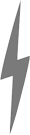
\includegraphics{simon/resources/lighting.png}}};
    \node at (12.5,112) {\resizebox{1.3mm}{!}{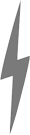
\includegraphics{simon/resources/lighting.png}}};
    \node at (22.5,112) {\resizebox{1.3mm}{!}{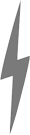
\includegraphics{simon/resources/lighting.png}}};
    \node at (32.5,112) {\resizebox{1.3mm}{!}{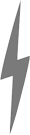
\includegraphics{simon/resources/lighting.png}}};
    \node at (42.5,112) {\resizebox{1.3mm}{!}{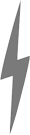
\includegraphics{simon/resources/lighting.png}}};
    \node at (52.5,112) {\resizebox{1.3mm}{!}{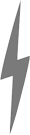
\includegraphics{simon/resources/lighting.png}}};
    \node at (62.5,112) {\resizebox{1.3mm}{!}{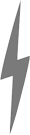
\includegraphics{simon/resources/lighting.png}}};
    \node at (72.5,112) {\resizebox{1.3mm}{!}{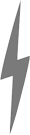
\includegraphics{simon/resources/lighting.png}}};
    \node at (82.5,112) {\resizebox{1.3mm}{!}{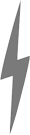
\includegraphics{simon/resources/lighting.png}}};
    \node at (92.5,112) {\resizebox{1.3mm}{!}{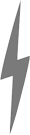
\includegraphics{simon/resources/lighting.png}}};
  \end{axis}
\end{tikzpicture}
\caption{Arcing Activity}
\labfig{arcing-activity}
\end{figure}

\begin{figure}[h!]
\begin{tikzpicture}
  \begin{axis}[
    xmin=0,
    xmax=3.75,
    ytick = none,
    xtick distance = 1,
    width = \textwidth,
    height = 5cm,
    axis y line = left,
    axis x line = middle,
    xlabel = \(t\) in \(ms\),
    %ylabel = sound pressure,
    scaled ticks = false,
    x filter/.code=\pgfmathparse{#1 * 1000},
    area style,
    ]
    \addplot+[draw=black, fill=gr10] table [x=t, y=disp, col sep=comma, mark=none]{simon/resources/signal.csv};
  \end{axis}
\end{tikzpicture}
\caption{Sound Pressure}
\labfig{sound-pressure}
\end{figure}

\begin{figure}[h!]
\begin{tikzpicture}
  \begin{axis}[
    xmode = log,
    xmin = 300,
    xmax = 22000,
    ymax = 60,
    ytick = {0},
    yticklabels = \empty,
    xticklabels = \empty,
    extra x ticks = {500,1500,2500,10000},
    width = \textwidth,
    height = 5cm,
    axis y line = left,
    axis x line = middle,
    tick align = inside,
    log ticks with fixed point,
    % 1000 sep = {\,},
    xticklabel style={/pgf/number format/.cd,1000 sep = {\;},fixed},
    scaled ticks = false,
    xlabel = \(f\) in \(Hz\),
    %ylabel = magnitude
    ]
    \addplot+[ycomb, draw=black, mark options={gr40}] table [x=f, y=mag, col sep=comma]{simon/resources/fourier.csv};
  \end{axis}
\end{tikzpicture}
\caption{Frequency Magnitude}
\labfig{frequency-magnitude}
\end{figure}

\todo{Add section on how to play multiple tones}

a

\subsection{Analog modulation}

.

\setchapterstyle{kao}
\setchapterpreamble[u]{\margintoc}

\chapter{Design and Simulation} % How I thought it was going to work
\labch{tc-design-and-simulation}

\textbf{Disclaimer:} This process was a lot more length and tedious than depicted in the following chapter. It mostly consisted of trial and error, which started with an more or less educated guess and ended in cluelessness and despair. But those errors don't add a lot of value to understanding the topic, so I won't go into much detail.

\section{The Coils}

The goal was to design an air coil with a resonant frequency of 4MHz. This frequency was chosen, since it is high enough to work well with an class E amplifier, but low enough to not run into too many RF related problems. It was also already known to have worked with a few other class E tesla coils.

\subsection{Rough Estimation of the Secondary Coil}

The inductance of a single-layered air solenoid coil can be calculated with

\begin{equation}\label{eq-inductivity}
    L = \mu_0 \frac{N^2 A}{l}
\end{equation}

The parasitic capacitance, depending on its length \(l\) and its diameter \(D\) can be calculated with\sidecite{self-capacitance}

\begin{equation}\label{eq-parasitic-capacitance}
    C_L = \frac{4\varepsilon_0}{\pi} \cdot l \cdot \left( 1 + 0.8249 \frac{D}{l} + 2.329 \left(\frac{D}{l}\right)^{1.5}\right)
\end{equation}

Defining the length to diameter ratio of the coil to be 4, and \(d_w\) to be the diameter of the wire, both formulas can be rewritten to only depend on \(l\) and \(d_w\). 

\begin{equation}
    L = \mu_0 \frac{l^3\ \pi}{32 d_w^2}
\end{equation}

\begin{equation}
    C_L = \frac{4\varepsilon_0}{\pi} \cdot l \cdot 1.49735
\end{equation}

Those equations can then be set into the formula for the resonant frequency of an LC circuit.

\begin{equation}
    f = \frac{1}{2\pi \cdot \sqrt{0.1872 \cdot \dfrac{1}{d_w^2} \cdot \mu_0 \varepsilon_0 \cdot l^4}}
\end{equation}

Rearranging the equation to \(l\)

\begin{equation}
    l = \frac{1}{\sqrt[\scalebox{1}{4}]{4\pi^2 f^2 \cdot0.1872 \cdot \dfrac{1}{d_w^2} \cdot \mu_0 \varepsilon_0}}
\end{equation}

With a frequency of 4MHz and a wire diameter of 0.35mm, the length of the coil turns out to be around 100mm and the diameter therefore around 25mm.

Due to the materials available, a 30 mm tube was used to wind the wire around. By using equation \ref{eq-inductivity} and \ref{eq-parasitic-capacitance}, an equation can be derived, which describes the relationship of all relevant variables.

\begin{equation}
    f = \frac{1}{2\pi \dfrac{D}{d_w} \sqrt{\mu_0 \varepsilon_0 \left( l^2 + 0.8245 D l + 2.329 D^{1.5} \sqrt{l} \right)}}
\end{equation}

Using Wolfram Alpha to solve this equation for \(l\) with a \(D\) of 30 mm gives a length of 112 mm.
% 4000000 = 1/(2π(0.03/0.00035)Sqrt[11.1265e-18*(Power[x,2]+0.8245*0.03*x+2.329*Power[0.03,1.5]*Sqrt[x])]) solve for x

\subsection{Tuning the Secondary Coil}\label{TC-tuningTheSecondary}

Tuning the coil to the correct frequency is essential, because all calculated values from above are highly idealized. For example, equation \ref{eq-parasitic-capacitance} is said to have a standard deviation of \(\sigma_{CL} \text{in pF} = 3.6 \cdot D\), which leads to a standard deviation of around 116 kHz of the resonant frequency of the coil. In addition, the relative permeability and permittivity factor of the carrier material are not taken into consideration in the calculations.

The coil was tuned by exciting the base of the secondary coil with a sinusoidal voltage. An oscilloscope probe, formed into a current loop, was placed near the top of the coil. The closer the excitation frequency was to the resonant frequency of the coil, the higher the measured voltage on the oscilloscope. The frequency, at which the measured voltage was at its maximum, was the resonant frequency of the coil. By adding or removing windings, the resonant frequency could be lowered or raised, until it exactly matched 4MHz\sidenote{In order to avoid adding windings, which was more tedious than removing them, the coil was wound around 10\% longer than calculated}.\todo{Add how close the original calculations were}

\subsection{Designing the Primary Coil} \label{TC-designingThePrimary}

The primary coil offers a lot of design freedom and flexibility, but this also means, that there is no \enquote{correct} or \enquote{ideal} design, but only one, which has been observed to work well. It mostly comes down to optimizing the coupling coefficient between the two coils. If it's too low, not enough energy will be transferred to the secondary, but to raise it, the coils have to be moved closer together which leads to flashover, due to too low insulation. \todo{Test tesla coil with coupling factor of 0.10 to 0.15}% Source: book page 55
This limitation can be bypassed by making the primary coil smaller at the bottom, where the voltage is higher and larger at the top, where the voltage is higher. This results in the well-known conical shape known from many tesla coils.\todo{Maybe add marginfigure with small illustration}



\section{The Class-E Stage}

\section{The Interrupter}
\chapter{Practice and Measurements} % How it actually works
\labch{tc-practice-and-measurements}

\section{The Coil}

\section{The Class-E Stage}

\section{The Interrupter}

% Todo
% 2.2   The Class-E Stage
% 3.x Practice
% 4.x Future Improvements

\pagelayout{wide} % No margins
\addpart{Design and Building}
\pagelayout{margin} % Restore margins
\setchapterstyle{kao}
\setchapterpreamble[u]{\margintoc}

\setcounter{chapter}{9}

%%% For material score
\newcommand{\outerradius}{1cm}
\newcommand{\innerradius}{.75cm}
\newcommand{\barlength}{2cm}
\newcommand{\barheight}{1.5mm}
\newcommand{\barypos}[1]{- \outerradius + #1 * \outerradius / 2 - \outerradius / 4 - \barheight / 2}

\newcommand{\materialscore}[6]{
\begin{tikzpicture}

    \fill[gr20] (0,0) circle (\outerradius);
    \fill[gr50] (0,0) -- (0, \outerradius)
      arc (90:90-36*#2:\outerradius) -- (0,0);
    \fill[white] (0,0) circle (\innerradius);

     \node[gr70] at (\outerradius + 5mm, \barypos{4} + \barheight / 2) {\faIcon{magnet}};
     \fill[gr20] (\outerradius + 9mm, \barypos{4}) rectangle ++(\barlength, \barheight);
     \fill[gr50] (\outerradius + 9mm, \barypos{4}) rectangle ++(\barlength * 0.1 * #3, \barheight);

    \node[gr70] at (\outerradius + 5mm, \barypos{3} + \barheight / 2) {\faIcon{fire}};
    \fill[gr20] (\outerradius + 9mm, \barypos{3}) rectangle ++(\barlength, \barheight);
    \fill[gr50] (\outerradius + 9mm, \barypos{3}) rectangle ++(\barlength * 0.1 * #4, \barheight);

    \node[gr70] at (\outerradius + 5mm, \barypos{2} + \barheight / 2) {\faIcon{euro-sign}};
    \fill[gr20] (\outerradius + 9mm, \barypos{2}) rectangle ++(\barlength, \barheight);
    \fill[gr50] (\outerradius + 9mm, \barypos{2}) rectangle ++(\barlength * 0.1 * #5, \barheight);

    \node[gr70] at (\outerradius + 5mm, \barypos{1} + \barheight / 2) {\faIcon{eye}};
    \fill[gr20] (\outerradius + 9mm, \barypos{1}) rectangle ++(\barlength, \barheight);
    \fill[gr50] (\outerradius + 9mm, \barypos{1}) rectangle ++(\barlength * 0.1 * #6, \barheight);

    \foreach \l in {1,...,4}{
      \foreach \p in {1,...,9}{
        \draw[gr20, ultra thick] (\outerradius + 9mm + \barlength / 10 * \p, \barypos{\l}) -- ++(0, \barheight);
      }
    }

    \foreach \a in {0,36,72,...,360}{
      \draw[gr20, ultra thick] (\a+18:\innerradius) -- (\a+18:\outerradius);
    }

    \node at (\outerradius / 2 + \barlength / 2, \outerradius * 1.25){\large{\textbf{#1}}};
\end{tikzpicture}}

\chapter{Casing}

% Since the tesla coil is intended as a consumer product, the casing plays an important role for its appearance. But apart from optics, there are a lot of safety hazards, which the casing has to account for. Most notably is the very real fire risk, which goes along playing with open plasma.

% Another point to note is, that the casing was build with modularity in mind. This enables to repair 
It might seem like the casing is not very significant, even though the design and function of all kinds of device's exteriors is crucial. The simplest of casings often have multiple design stages and variations with different advantages. When designing something as complex and difficult as a tesla coil, the casing is even more rigorous to construct. 


\section{Concept design}
\label{sec:concept-design}

There are four main parts that are essential to consider while constructing the tesla coil - the primary coil, the secondary coil, the \gls{pcb}, and the top electrode. Those can be placed in any way possible, but there is a reasonable standard practice for their placement, especially for the coils and the top electrode. 

\begin{figure}
    \centering
    %\missingfigure
    %\includegraphics{}
    \caption{Concept design}
    \label{BD-envision}
\end{figure}

As seen above, the secondary coil is perpendicular, and the primary coil is angled at 30°\sidenote{The primary coil design choices have already been explained in the previous part at the end of \ref{sec:designing-the-primary}} to the horizontal. This is the easiest way to calculate and most practical way to design the secondary. The placement for the top electrode seems very obvious, but there is an explanation. If the arching point of the electrode is placed further away from the secondary, the behavior of the coils will become less predictable the more distance is between them. So the most practical placement is in the middle and a few centimeters above the secondary coil.

Technically the \gls{pcb} can be placed anywhere\sidenote{There should be a reasonable distance between the PCB and the coils to ensure that the electrical field does not interfere with the circuitry.} as long as it can be connected to the coils. However, to make transportation the easiest, the casing for the \gls{pcb} should be right beneath the coils. This way, everything needed stays in one place. 

\section{Materials}

Deciding which materials to use is also a tedious task because there are a lot of details and possibilities that have to be considered when designing a tesla coil. Many factors determine the best working material, most affecting the coils directly and therefore being unsuitable, but others are scrapped because of their low availability or costly construction.

\subsection{Metals}
\label{subsec:materials-metals}

Metal is a popular choice for building high-grade casings because of its low price and good machinability. However, metals are rather unsuitable for a tesla coil, mainly because of their electrical conductivity, which would pose an unnecessary safety risk to the user when touched. On one side, because some internal connection error could be lethal in the worst case, but also because if not properly grounded, static electricity could build up in the casing and shock everyone touching it. Another critical factor is that metals have very high permeability, weakening any magnetic field. This would not be a big problem for the \gls{pcb} enclosure but would certainly cause issues when used around the primary or secondary coil.

\subsection{Woods}

One material that is not often used for casings, especially for commercial products, is wood, mainly because it is more expensive and harder to work with than metal. This tesla coil is not like any device, but wood is still not a good option, mainly because the top electrode emits a high-temperature spark which could inflame the wooden casing. Making the casing for only the board wooden would not work either because if the capacitance of the secondary coil changes, the driver operates outside of its ideal conditions and dissipates a lot of energy as heat, potentially inflaming the wood.

\subsection{Glass}

Glass is an electrical insulator, so it would not interfere with the magnetic field, has very high-temperature resistance, and has a polished look. It also comes in various opacities, and surface finishes making the casing very customizable. The main disadvantage of glass is its high production costs. Due to the tesla coil not being commercially produced, this kind of casing is unsustainable.

\subsection{Plastics}

\glsunset{pvcp}\glsunset{pmma}\glsunset{pvcu}\glsunset{ptfe}
The only remaining option for the type of casings material would be plastic. However, plastic is not plastic. The two types of plastic with the highest availability, in this case, would be \gls{pvcp} and \gls{pmma}\sidenote{also commercially known as acrylic glass or plexiglass}. There is also \gls{pvcu}, but given that it is harder to process and also less available, \gls{pvcp} is preferred. \gls{pvcp} would be a lot better than \gls{pmma} when it comes to cost and availability, but it cannot provide the suitable characteristics for the tesla coil. One problem with \gls{pvcp} is its water absorption because due to water's diamagnetic properties, it heats up in an oscillating magnetic field, i.e., it is wasting energy. \gls{pvcp}s water absorption over 24 hours lies at a maximum of 1\% of its total weight. \gls{pmma}, in comparison, has an absorption of 0.4\% at max. On the other hand, \gls{pvcu} has an even more ideal water absorption at 0.1\%. The casing should not be out of \gls{pvcp} or \gls{pvcu} because of its poor temperature resistance, which starts to deform at around 60°C, while \gls{pmma} only starts at about 100°C. \gls{pmma} is not ideal in any way, but due to its easy availability and better properties, it was chosen for the casing. 

The ideal plastic would be \gls{ptfe}\sidenote{also commercially known as Teflon}, which has a maximum of 0.01\%, a tenth better than \gls{pvcu}. The temperature resistance is also better than \gls{pmma} because it can be used at a working temperature of 280°C\sidecite{blue-bible}. \gls{ptfe} was not used as a casing because it was unavailable, but it might be considered in a future build.  

\todo{Welche veraussetzung die materialien haben müssen und warum gewisse nicht in frage kommen. Berechnungen auch Permeabilität \& Permittivität
https://omnexus.specialchem.com/polymer-properties/properties/water-absorption-24-hours einbinden}

\subsection{Conclusion}

In figure \ref{fig:material-score}, all previously discussed materials are given a subjective score from 1 to 10 in the four most important categories. The score in the circle is then determined by the average points of these categories, quickly visualizing which material is best suited for the tesla coil. Both \gls{ptfe} and \gls{pmma} have the same total score, but as already mentioned above, \gls{ptfe} wasn't used because of the low availability.  

\begin{figure}[h!]
    \centering
    \begin{tabular}{cc}
      \materialscore{Metal}{4}{1}{8}{6}{3} & \materialscore{Wood}{5}{6}{2}{7}{6} \\
      \materialscore{Glass}{7}{9}{9}{1}{10} & \materialscore{PMMA}{8}{8}{6}{9}{7} \\
      \materialscore{PVC-U}{7}{9}{6}{9}{5} & \materialscore{PTFE}{8}{10}{7}{8}{6} \\
      \multicolumn{2}{l}{
      \begin{tabular}{cl}
        \\
        {\color{gr70}\faIcon{magnet}} &  Magnetic and Electrical Properties \\
        {\color{gr70}\faIcon{fire}} &  Temperature resistance \\
        {\color{gr70}\faIcon{euro-sign}} &  Machinability and cost \\
        {\color{gr70}\faIcon{eye}} &  Optics
      \end{tabular}}
    \end{tabular}
    \caption{Bottom text}
    \label{fig:material-score}
\end{figure}



\section{Structure for the Coils}

As mentioned in section \ref{sec:concept-design}, both coils have a fixed position and shape, but to ensure this, the casing has to be built based on them. The secondary is easy to support, but the primary has a unique shape that has to be kept in form. 

\subsection{Primary Coil}

The primary coil's holding structure consists of six supports arranged in a hexagonal way. Every support is a triangular-shaped slope with an angle of 30°, on top of which the primary coil rests. In order to keep the primary coil in place, small half-circles have been cut out for every turn. However, to keep the coil's shape, the ten slots on each support have to be shifted up by one-sixth of the distance between each other.

\begin{figure}[h!]
    \centering
    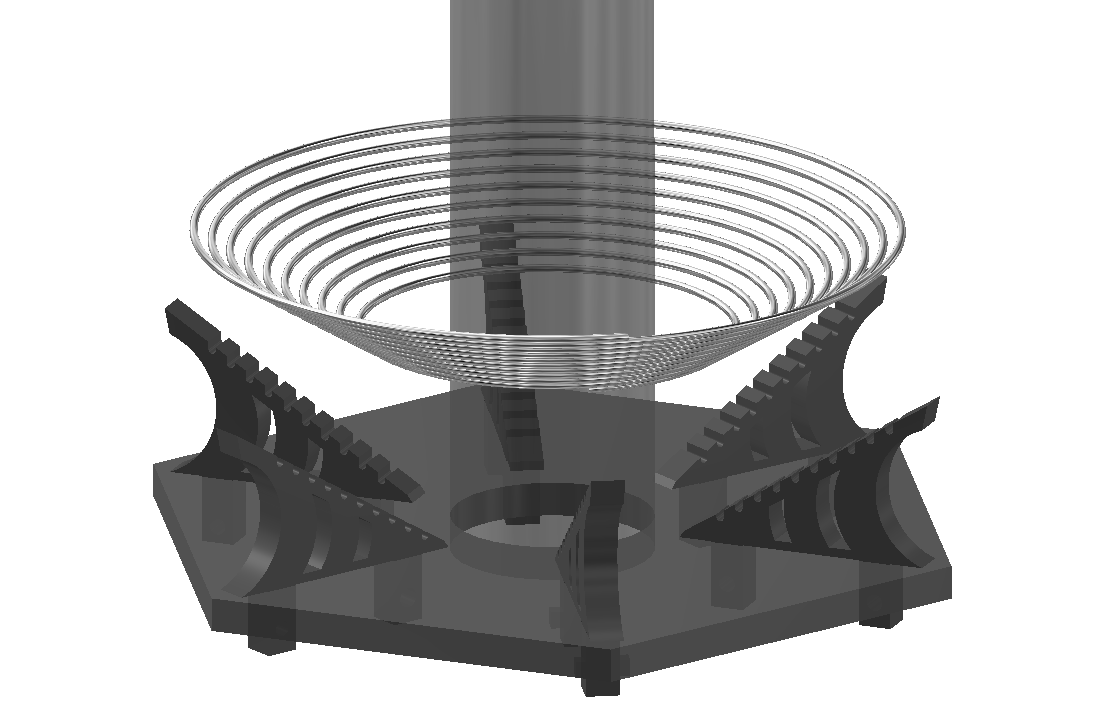
\includegraphics[width=1\textwidth]{kassandra/resources/endeMeinerHoffnung.png}
    \caption{3D view of the primary supports}
    \label{fig:primary-supports}
\end{figure}

To avoid gluing the supports to the base plate, a bolt was used to keep it in place, as shown in figure \ref{fig:stayer}. This mechanism was mainly designed for testing purposes as it is easier to assemble and disassemble. In a possible future version or commercial release, it would be safer if the supports were glued on. Also, as shown, the supports have a unique design. This was mostly done to make them look elegant and not stand out too much. That makes them lighter, but given that the supports are just a tiny fraction of the tesla coil's weight, it does not make much difference.

\begin{figure}[h!]
    \begin{subfigure}{0.5\textwidth}
        \centering
        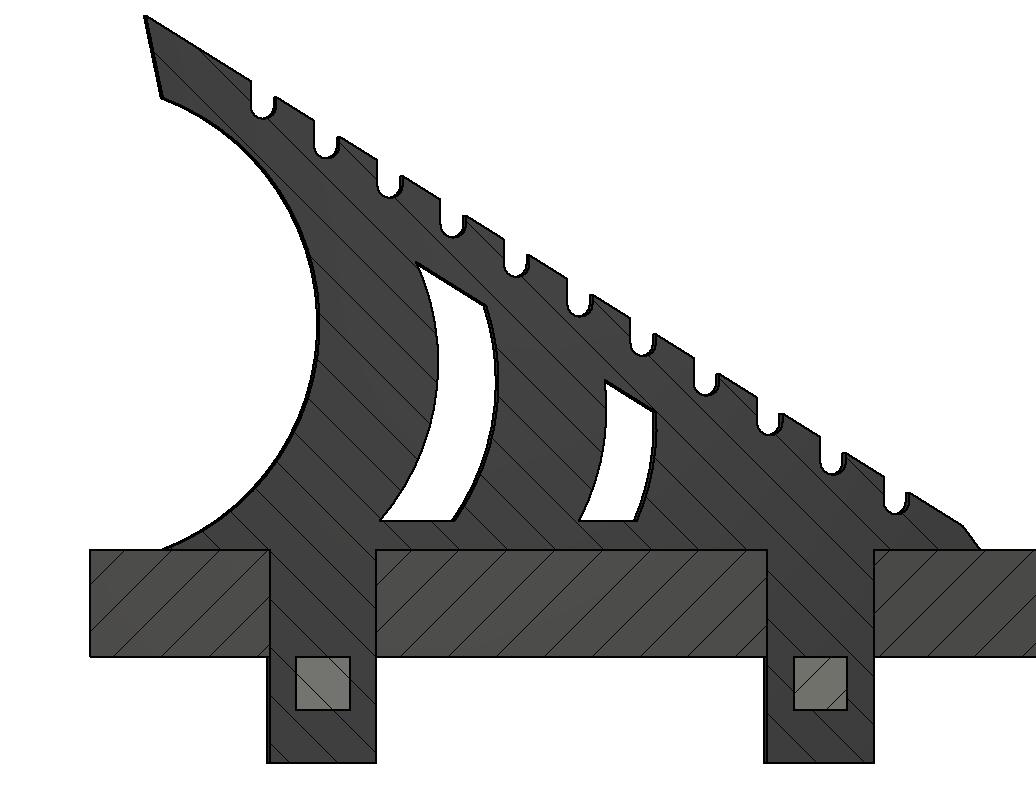
\includegraphics[width=\textwidth]{kassandra/resources/endeMeinerHoffnungInSemi2DStayer.PNG}
    \end{subfigure}%
    \begin{subfigure}{0.5\textwidth}
        \centering
        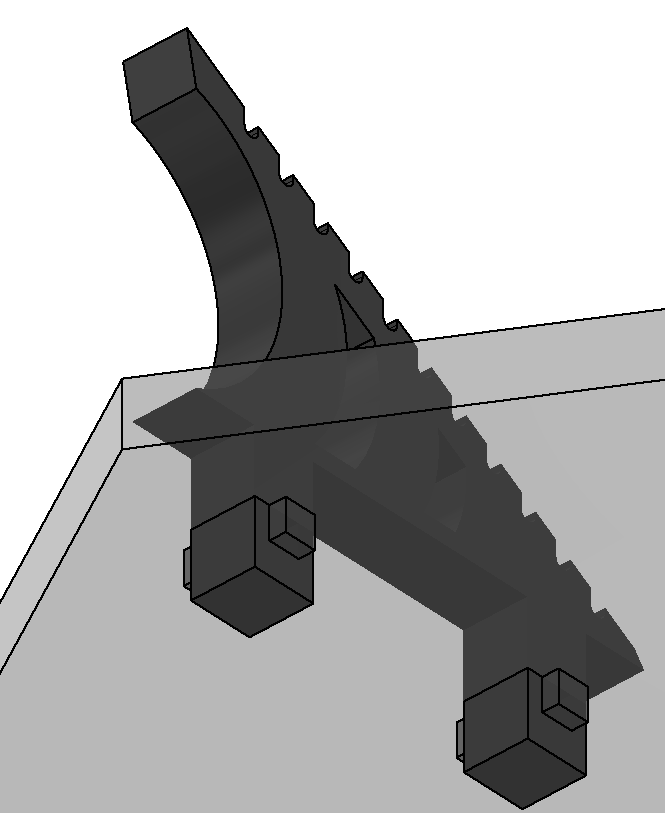
\includegraphics[width=0.7\textwidth]{kassandra/resources/endeMeinerHoffnungIn3DStayer.PNG}
    \end{subfigure}
    \centering
    \caption{Fastening of the supports}
    \label{fig:stayer}
\end{figure}

\subsection{Secondary Coil}

The core of the secondary coil was one of the easier parts to design because it essentially just consists of a 30mm \gls{pmma} tube with a thickness of 3mm. A few millimeters from the top of the tube, a small hole was drilled to guide the wire to the inside and connect it to the top electrode. The 330 turns of 0.35mm wire were then wound by hand and then coated with protective and insulating varnish to prevent the wire from loosening and cross-arcing to occur.

\todo{Das Gerüst für die zwei spulen. Stayer Desgin und funktion.}

\section{Top Electrode}

Technically the tesla coil would also work without a top electrode by simply using the end of the secondary coil's wire as the arcing point. however, given that the wire of the secondary has a small diameter and is made of copper, it would likely melt or at least start to deform when it emits a spark. To ensure the arcing point stays intact, the wire is connected to another material - in this case, a welding electrode made of a tungsten alloy. 

The holder that keeps the electrode at the top of the coil is made of two parts. As seen in figure \ref{fig:top-electrode}, the first is two copper pieces that are kept together with a thread, and in between, the wire of the secondary is clamped. There are also two notches on each to enable fastening and opening with a flat wrench. To mount the tungsten electrode, a press fit was drilled into the top surface of the copper piece. 

The second part is a \gls{pmma} piece with another fit at the top for the copper piece. On one side, there is also a gap to direct the wire of the secondary to the inner part. 

\begin{marginfigure}[-8cm]
    \centering
    \includegraphics[width=0.7\textwidth]{kassandra/resources/endeMeinerHoffnungFürBlitz.PNG}
    \caption{Mounting of the top electrode}
    \label{fig:top-electrode}
\end{marginfigure}

\subsection{It's not a Bug, it's a Feature}

Because the tesla coil driver was very underdesigned, the plasma flame forming on the top electrode was very small and often had to be ignited and stabilized by another conductor held close to it. This was realized by placing a second, ancillary electrode over to the main electrode. This ancillary electrode is held by a canopy-like structure, resting on three \gls{pmma} rods. It was press fitted into a flat copper cylinder, which was loosely screwed into the cap. This way, its height and the gap between the two electrodes could be changed by turning the ancillary electrode. 

\begin{marginfigure}[-3cm]
    \centering
    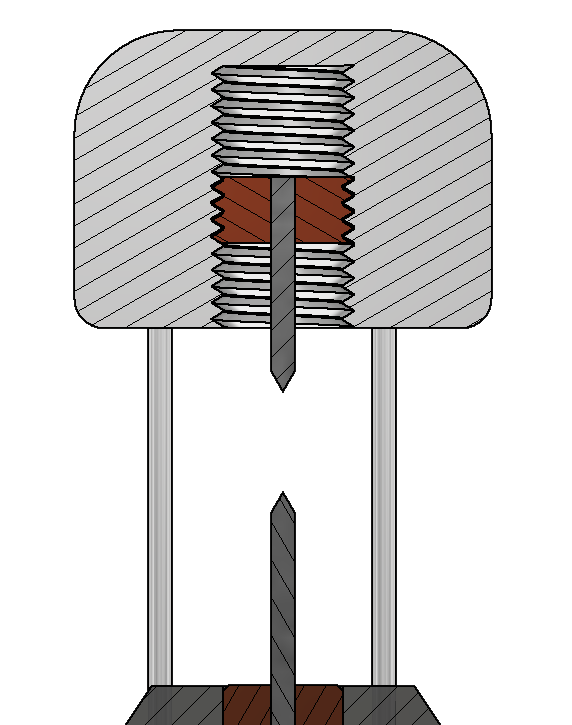
\includegraphics[width=\textwidth]{kassandra/resources/mirGehtsSuperDanke.png}
    \caption{Mounting of the ancillary electrode}
    \label{fig:ancillary-electrode}
\end{marginfigure}

To further examine the effect of the material of the cap, three different versions have been made. One out of \gls{pmma} and two out of Aluminium, one of which is as smooth as possible and one as pointy as possible.

\begin{figure}[h!]
    \centering
    \label{fig:caps}
    \begin{subfigure}[b]{0.4\textwidth}
        \centering
        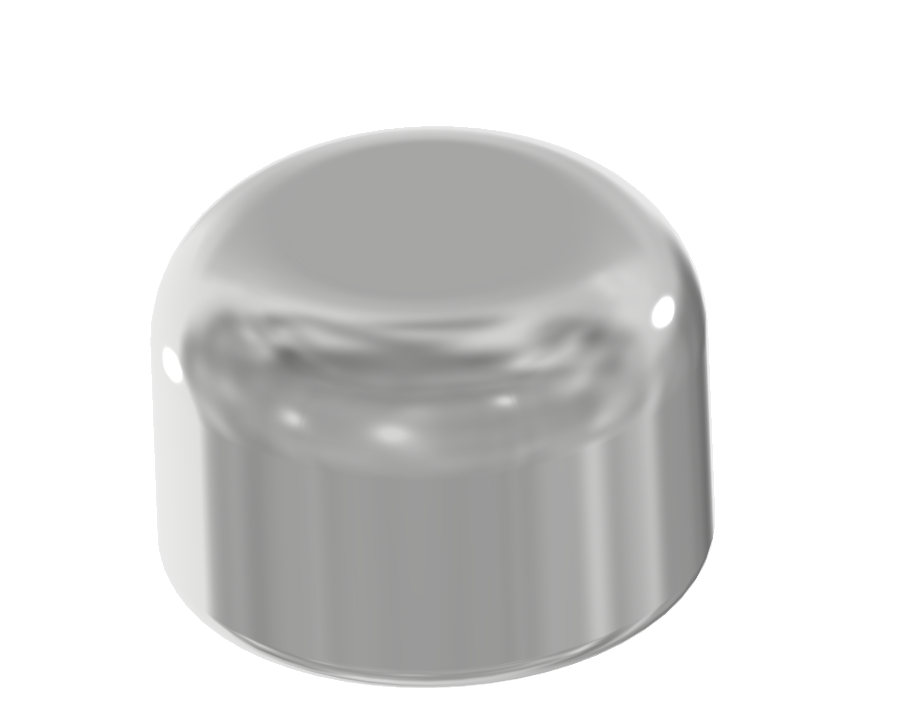
\includegraphics[width=0.9\textwidth]{kassandra/resources/mirGehtsSuperDankeSmooth.png}
    \end{subfigure}
    \hfill
    \begin{subfigure}[b]{0.4\textwidth}
        \centering
        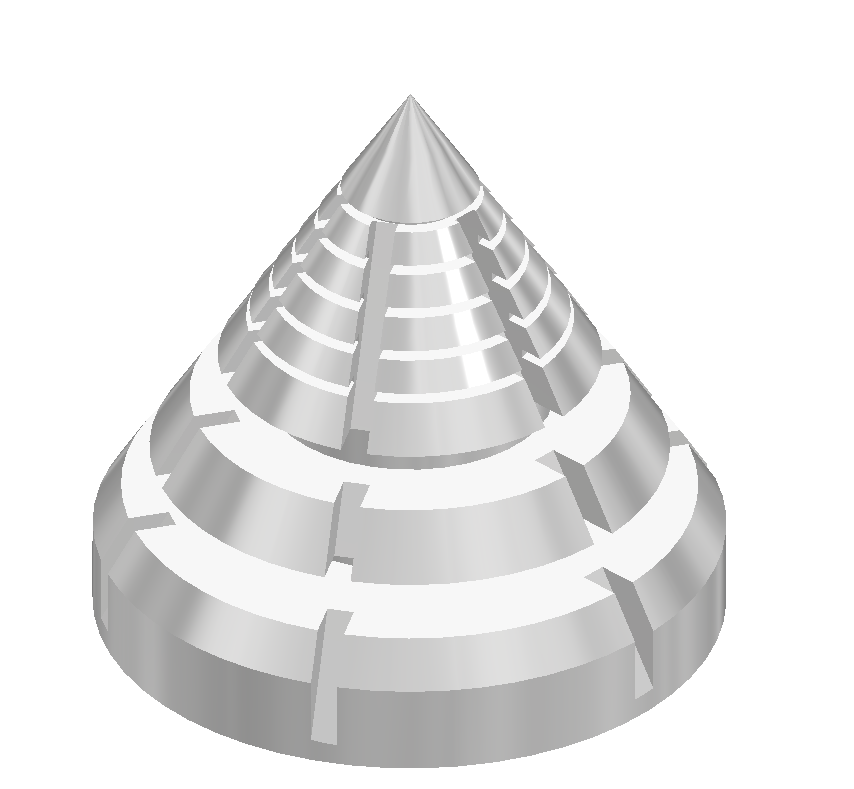
\includegraphics[width=0.9\textwidth]{kassandra/resources/mirGehtsSuperDankeEdgy.png}
    \end{subfigure}
    \caption{Smooth and Pointy Cap}
\end{figure}

While in section \ref{subsec:materials-metals}, it was explained that metals pose a safety hazard, this is not entirely true for the secondary side of the tesla coil. Despite the high voltages of up to several kilovolts present at the top electrode, it is relatively safe to touch. This is because as soon as a low-resistance path to ground, like a human, opens for the current, the voltage drops to a very low level, which means that the resulting current cannot do any harm besides the usual burned skin.

\section{PCB Enclosure}

The general placement of the \gls{pcb}, being right beneath the coils, was already addressed in section \ref{sec:concept-design}. The platform where the secondary coil and the supports for the primary coil are mounted was already designed and chosen to be hexagon-shaped, mainly because it works the best with the six supports. Again, the prototype has the platform resting on top of six pillars to keep everything as modular as possible. The prototype also has only the most essential features and only consists of a framework, this also makes it easier to access the inside of the \gls{pcb} enclosure. The final design would be completely closed off, and the platform would be glued on as with the primary coil’s supports.

\subsection{PCB}

The hexagonal \gls{pcb} was placed in the center of the enclosure right under the secondary, mostly to balance the design. To ensure that the circuit can also give off heat on the bottom side, it cannot be mounted directly onto the enclosure and therefore has to be raised by a few millimeters. This is done by six steps onto which the \gls{pcb} is screwed. 

\subsection{Connections and Things to Press}

To provide the necessary power and the MIDI-Interrupter signal to the PCB as well as the ability to be turned on and off without being plugged out, one side of the PCB enclosure has been dedicated as a control panel. To provide the necessary power, a 5.5 x 2.1 mm barrel plug was used because of its widespread usage. To connect the fiber optic cable, the phototransistor has been mounted directly into the casing, so it is still accessible from the outside. Additionally, a keyswitch\sidenote{This way, only authorized people are able to turn on the tesla coil and feel important} is used to turn on the power, and an ON-OFF-ON switch either routes the output of the phototransistor for interrupted operation, a constant 12V signal for continuous operating, or a 0V signal for no operation to the interrupt input.

\chapter{Printed Circuit Board}

\glspl{pcb} playe an essential role in this project. Breadboards and other prototyping techniques tend to cause issues with parasitic inductances and capacitances and do not work with \gls{smd} components, so \glspl{pcb} were the only way to build up the circuits. Once a \gls{pcb} has been produced, it works reliable and usually does not add any erratic effects. On the downside, however, \glspl{pcb} take a lot of time to design, etch, and solder, and once they are manufactured, they are very inflexible. This means that a new \gls{pcb} had to be made for every prototype..

\section{Component Selection}

Because almost none of the needed components were on hand in the school laboratories, they had to be ordered online. Due to the unique requirements of some parts, like the MOSFET or the \gls{vco}, they were rather hard to find and either very costly or came in an impractical package.

Since all the essential components were only available as \glspl{smd}, most other components were also shifted to \gls{smt} for consistency.


\subsection{ICs}

Most ICs were only available in one package and did not leave much flexibility. The MOSFET driver, \gls{vco}, latch, AND gate, and MOSFET for the phototransistor came in standard SOT and SOIC packages which were easy to solder since they have the pins on their side. The class-E MOSFET and the voltage regulator were somewhat troublesome because their packages had a big metal area on the underside, only indented for one-time reflow soldering. Unfortunately, the class-E MOSFET still needed to be replaced multiple times during the testing process.

\subsection{Passive Elements}

All capacitors and resistors have been ordered in a 0805 package because it is not too big but just big enough to be easy to work with. The small size compared to \glspl{thd} does, however, negatively affect the power rating of resistors and the voltage rating of capacitors, so it had to be made sure that they still operated within the safe operating range. For the capacitors, X7R devices had been chosen, which means that their operating temperature ranges from -55\textdegree C to 125\textdegree C with at most 15\% capacitance change over this range\textsuperscript{\sidecite{epci}}.

%\subsection{Connectors}



% Took some time to find all components

% SMD
% This is the final list of selected components:

\begin{tabular}{@{}lll@{}}
    \toprule
    \textbf{Part name} & \textbf{Footprint} & \textbf{Description}\\\midrule
    BSC12DN20N & PG-TDSON-8 & MOSFET\\
    IX4310 & SOT-23 & MOSFET driver\\
    LTC1799 & SOT-23 & Oscillator\\
    LM7805 & TO252 & Voltage regulator\\
    PKE3316 & Custom THT & boost converter\\
    74HC72 & SOIC127 & D-type latch\\
    TC7SZ08F & SOT-32 & AND gate\\
    RUM001L02 & SOT-723 & MOSFET\\
    47\(\mu\)H choke & Custom SMD &\\
    Various Capacitors & 0805 &\\
    Various Resistors & 0805 &\\
    Potentiometers & PT-10&\\
    Fuse 250mA & 1206 &\\
    Clamp & ? &\\
    Connector & CON06 &\\
    \bottomrule
\end{tabular}

\section{Physical arrangement}
\label{sec:physical-arrangement}

Two things about the placement of the electronics were already certain - that the class-E amplifier and its surroundings were placed in the center of the casing and that the connectors and controls had to be mounted on the side of the casing. The question is how to connect them. Using loose cables would quickly become unclear and cause noise to be picked up by the unamplified interrupter signal from the phototransistor. This could be solved by bundling all signals directly onto a \gls{pcb} and leading them to the main \gls{pcb} via a six pin flat ribbon cable. Additionally, this side board could amplify the interrupter signal to 12V to make it more resilient to induction. 


% Connection to the Coil
% Connection between the PCBs
% Connection to the Perpherals

\section{PCB Layout}

%\section{Manufacturing}

\pagelayout{wide} % No margins
\addpart{MIDI Interrupter}
\pagelayout{margin} % Restore margins
MIDI-Interrupter Zeugs

\appendix % From here onwards, chapters are numbered with letters, as is the appendix convention

\pagelayout{wide} % No margins
\addpart{Appendix}
\pagelayout{margin} % Restore margins

\chapter*{Special Thanks ...}

... to \textbf{Federico Marotta} for providing \enquote{kaobook}, the \LaTeX{} document class this thesis is built upon. It is licensed under the \href{https://www.latex-project.org/lppl/lppl-1-3c/}{LPPL-1.3c} and can be found on \href{https://github.com/fmarotta/kaobook}{github.com/fmarotta/kaobook}.

... to \textbf{Overleaf} for taking so long to compile documents, that we had plenty of time to reconsider our wording.

... to our headmaster \textit{Hofrat Günter Schweigler}. Well no, actually not.

... to some others too.

\pagebreak

%----------------------------------------------------------------------------------------

\backmatter % Denotes the end of the main document content
\setchapterstyle{plain} % Output plain chapters from this point onwards

%----------------------------------------------------------------------------------------
%	BIBLIOGRAPHY
%----------------------------------------------------------------------------------------

% The bibliography needs to be compiled with biber using your LaTeX editor, or on the command line with 'biber main' from the template directory

\defbibnote{bibnote}{Here are the references in citation order.\par\bigskip} % Prepend this text to the bibliography
\printbibliography[heading=bibintoc, title=Bibliography, prenote=bibnote] % Add the bibliography heading to the ToC, set the title of the bibliography and output the bibliography note

%----------------------------------------------------------------------------------------
%	NOMENCLATURE
%----------------------------------------------------------------------------------------

% The nomenclature needs to be compiled on the command line with 'makeindex main.nlo -s nomencl.ist -o main.nls' from the template directory

\nomenclature{SSTC}{Solid State Tesla Coil}
\nomenclature{CW}{Continuous wave}
\nomenclature{PCB}{Printed Circuit Board}

\renewcommand{\nomname}{Notation} % Rename the default 'Nomenclature'
\renewcommand{\nompreamble}{The next list describes several symbols that will be later used within the body of the document.} % Prepend this text to the nomenclature

%\printnomenclature % Output the nomenclature

%----------------------------------------------------------------------------------------
%	GLOSSARY
%----------------------------------------------------------------------------------------

% The glossary needs to be compiled on the command line with 'makeglossaries main' from the template directory

\newglossaryentry{computer}{
	name=computer,
	description={is a programmable machine that receives input, stores and manipulates data, and provides output in a useful format}
}

% Glossary entries (used in text with e.g. \acrfull{fpsLabel} or \acrshort{fpsLabel})
%          {label} {short} {long}
\newacronym{pcb}   {PCB}   {Printed Circuit Board}
\newacronym{ic}    {IC}    {Integrated Circuit}
\newacronym{smd}   {SMD}   {Surface Mount Device}
\newacronym{smt}   {SMT}   {Surface Mount Technology}
\newacronym{thd}   {THD}   {Through Hole Device}
\newacronym{tht}   {THT}   {Through Hole Technology}

% This groups all entries alphabetically
% \setglossarystyle{listgroup} % Set the style of the glossary (see https://en.wikibooks.org/wiki/LaTeX/Glossary for a reference)
\printglossary[title=Special Terms, toctitle=List of Terms] % Output the glossary, 'title' is the chapter heading for the glossary, toctitle is the table of contents heading

%----------------------------------------------------------------------------------------
%	INDEX
%----------------------------------------------------------------------------------------

% The index needs to be compiled on the command line with 'makeindex main' from the template directory

\printindex % Output the index

\pagecolor{black}
\newpage
a

\end{document}
